%%%%%%%%%%%%%%%%%%%%%%%%%%%%%%%%%%%%%%%%%% Preamble %%%%%%%%%%%%%%%%%%%%%%%%%%%%%%%%%%%%%%%%%%

\documentclass{assignment}
\usepackage[pdftex]{graphicx} % FIGURAS
\usepackage{xcolor}
\definecolor{LightGray}{gray}{0.95}
\usepackage[letterpaper, margin = 2.5cm]{geometry} 
\usepackage[T1]{fontenc} 
\usepackage{amsmath, amsfonts, amssymb, mathtools} 
\usepackage{hyperref, url}
\usepackage{fancyhdr}
\usepackage{listingsutf8}
\usepackage{tikz}
\usetikzlibrary{calc,trees,positioning,arrows,fit,shapes,calc}

\student{Yashashwin Karthikeyan, Roozbeh Ali}
\semester{Winter 2024}
\date{\today}

\courselabel{ECE108}
\exercisesheet{Assignment 7}{List Induction and Graph Theory}

\school{ECE 108 - Discrete Mathematics and Logic 1}
\university{University of Waterloo}

%% DOCUMENT

\begin{document}

\begin{problem}
  \section{Proof of Deletion}
  \subsection{Read}
  Yes.
  \subsection{Proof}
    \begin{flalign*}
        & \vdash \forall  xs \colon list(T_y). \; \forall x \colon T_y. \; \forall y \in del(x, xs). \; y \neq x. &\\
    \end{flalign*}
    By list induction on goal, \\\\ 
    \emph{\bf{Subproof 1 (Base case)}}
    \begin{flalign*}
        & \vdash \forall x \colon T_y. \; \forall y \in del(x, [ \; ]). \; y \neq x. &
    \end{flalign*}
    By forall-elim on goal,
    \begin{flalign*}
        & (1.1) x \colon T_y &\\
        & \vdash \forall y \in del(x, [ \; ]). \; y \neq x. &
    \end{flalign*}
    By subst. definition of $del$ into goal by logic,
     \begin{flalign*}
        & \vdash \; \forall y \in [ \; ]. \; y \neq x. &
    \end{flalign*}
    QED by empty-list membership axiom and logic. \\ \\
    \emph{\bf{Subproof 2 (Inductive step)}}
    \begin{flalign*}
        & (2.1) xs \colon list(T_y) &\\
        & (2.2) \forall x \colon T_y. \; \forall y \in del(x, xs). \; y \neq x. &\\
        & (2.3) x' \colon T_y. &\\
        & \vdash \forall x \colon T_y. \; \forall y \in del(x, push(x', xs)). \; y \neq x. &
    \end{flalign*}
    By forall-elim on goal,
    \begin{flalign*}
        & (2.4) x \colon T_y. &\\
        & \vdash \forall y \in del(x, push(x', xs)). \; y \neq x. &
    \end{flalign*}
    By forall-elim on (2.2) using (2.4),
    \begin{flalign*}
        & (2.5) \forall y \in del(x, xs). \; y \neq x.&
    \end{flalign*}
    By cases $x = x'$, $x \neq x'$, \\ \\ 
    \emph{\bf{Subproof 2.1 (Completeness)}}
    \begin{flalign*}
        & \vdash (x = x') \lor (x \neq x') &
    \end{flalign*}
    QED by logic. \\ \\
    \emph{\bf{Subproof 2.2 (Equality case)}}
    \begin{flalign*}
        & (3.1) x = x' &\\
        & \vdash \forall y \in del(x, push(x', xs)). \; y \neq x.&
    \end{flalign*}
    By rev subst. (3.1) into goal,
    \begin{flalign*}
        & \vdash \forall y \in del(x, push(x, xs)). \; y \neq x.&
    \end{flalign*}
    By subst. definition of $del$ into goal and the front axiom,
    \begin{flalign*}
        & \vdash \forall y \in del(x, pop(push(x, xs))). \; y \neq x.&
    \end{flalign*}
    By the pop axiom,
    \begin{flalign*}
        & \vdash \forall y \in del(x, xs). \; y \neq x.&
    \end{flalign*}
    QED by (2.5). \\ \\
    \emph{\bf{Subproof 2.2 (Inequality case)}}
    \begin{flalign*}
        & (4.1) x \neq x' &\\
        & \vdash \forall y \in del(x, push(x', xs)). \; y \neq x.&
    \end{flalign*}
    By susbt. definition of $del$ into goal, (4.1) and the front axiom,
    \begin{flalign*}
        & \vdash \forall y \in push(x', del(x, pop(push(x', xs)))). \; y \neq x. &
    \end{flalign*}
    By subst. pop axiom by logic, 
    \begin{flalign*}
        & \vdash \forall y \in push(x', del(x, xs)). \; y \neq x.&
    \end{flalign*}
    By subst. universal quantification over a list by logic,
    \begin{flalign*}
        & \vdash (front(push(x', del(x, xs))) \neq x) \; \land \; (\forall y \in pop(push(x', del(x, xs))). \; y \neq x.)&
    \end{flalign*}
    By subst. pop axiom and front axiom into goal by logic,
    \begin{flalign*}
        & \vdash (x' \neq x) \; \land \; (\forall y \in del(x, xs). \; y \neq x.) &
    \end{flalign*}
    QED by (4.1) and (2.5). \\ \\
    
    \emph{\bf{TA Notes}} \\ \\
    1. For the defn subst, we know the value in both cases by the equality assumptions, the front axiom, and the size being at least 1 for any return of the push function. \\ \\
    2. Universal quantification requires a set of non-zero size, and by definition any return of the push function has non-zero size. 
    
 \end{problem}

\begin{problem}
  \section{Categories of graphs}

  \subsection{List of nodes win}
  In undirected, directed and simple graphs, a list of nodes is advantageous for choosing a path. In undirected graphs, bi-directional edges play no importance, because a path cannot have repeat edges. Thus, a list of nodes effectively descibes a path for an undirected graph with minimal information. This similarly makes a list of nodes effective for simple graphs, because they are undirected. Directed graphs preserve direction by virtue of their edges being uni-directional. As such, a list of nodes would be preferrable in order to minimze the information required to make a graph.
  \subsection{List of edges win}
  A list of edges would be advantageous for a multigraph. Since nodes can be the  times, a list of edges is useful to identify the start and end point amongst potential parallel edges, and thus form a path.
  Choosing a path to be a list of edges would be useful for multigraphs. A core axiom of multigraphs are that 
  
\end{problem}

\begin{problem}
    \section{Graphs and injective functions}
    To represent an injective function, we move the endpoint of the edge $(x_4, y_3)$ to $y_4$, and delete the edge $(x_5, y_4)$. These operations have a total cost of 3. The following graph represents an injective function after the aforementioned operations are performed. \\
    \begin{figure}[htbp]
        \centering
             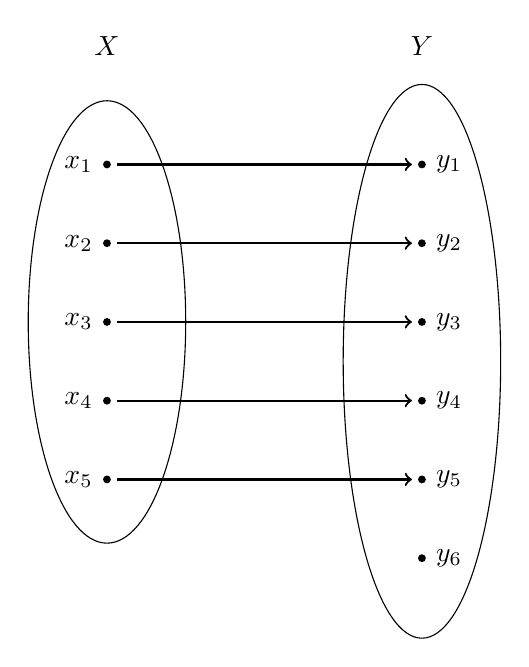
\begin{tikzpicture}[ele/.style={fill=black,circle,minimum width=.8pt,inner sep=1pt},every fit/.style={ellipse,draw,inner sep=-2pt}]
            
              \node at (0,6.5){$X$};
              \node at (4, 6.5){$Y$};
              
              \node[ele,label=left:$x_1$] (a1) at (0,5) {};    
              \node[ele,label=left:$x_2$] (a2) at (0,4) {};    
              \node[ele,label=left:$x_3$] (a3) at (0,3) {};
              \node[ele,label=left:$x_4$] (a4) at (0,2) {};
              \node[ele,label=left:$x_5$] (a5) at (0,1) {};
            
              \node[ele,,label=right:$y_1$] (b1) at (4,5) {};
              \node[ele,,label=right:$y_2$] (b2) at (4,4) {};
              \node[ele,,label=right:$y_3$] (b3) at (4,3){};
              \node[ele,,label=right:$y_4$] (b4) at (4,2) {};
              \node[ele,,label=right:$y_5$] (b5) at (4,1) {};
              \node[ele,,label=right:$y_6$] (b6) at (4,0) {};
            
              \node[draw,fit= (a1) (a2) (a3) (a4) (a5),minimum width=2cm] {} ;
              \node[draw,fit= (b1) (b2) (b3) (b4) (b5) (b6),minimum width=2cm] {} ;  
              \draw[->,thick,shorten <=2pt,shorten >=2pt] (a1) -- (b1);
              \draw[->,thick,shorten <=2pt,shorten >=2] (a2) -- (b2);
              \draw[->,thick,shorten <=2pt,shorten >=2] (a3) -- (b3);
              \draw[->,thick,shorten <=2pt,shorten >=2] (a4) -- (b4);
              \draw[->,thick,shorten <=2pt,shorten >=2] (a5) -- (b5);
             \end{tikzpicture}
\end{figure}
    
\end{problem}

\begin{problem}
    \section{DAG}
    In order to convert the graph into a directed acyclic graph (DAG), we must remove at minimum 1 edge. If we represent edges in (tail, head) tuples, then by deleting $(2, 6)$, we create a DAG. \\
        \begin{figure}[htbp]
        \centering
        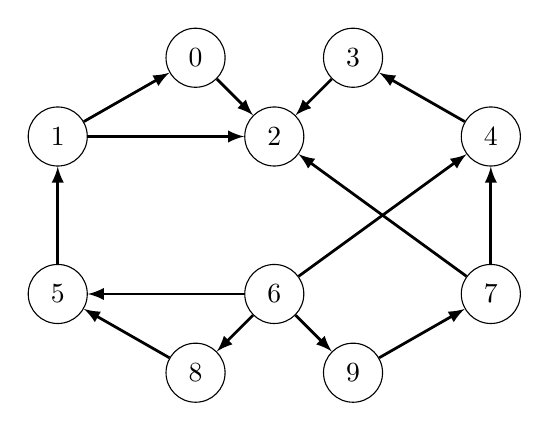
\begin{tikzpicture}
          [vertex/.style={circle,draw=black,fill=white},
           node distance=2cm and 2.75cm,
           on grid,
           minimum size = 0.75cm,
           >=latex
          ]
          \draw[gray!50];
          \node[vertex] (2) {2};
          \node[vertex,above left=1cm and 1cm of 2] (0) {0};
          \node[vertex,below=of 2] (6) {6};
          \node[vertex,left=of 6] (5) {5};
          \node[vertex,above=of 5] (1) {1};
          \node[vertex,below left=1cm and 1cm of 6] (8) {8};
          \node[vertex,above right=1cm and 1cm of 2] (3) {3};
          \node[vertex,right=of 2] (4) {4};
          \node[vertex,below=of 4] (7) {7};
          \node[vertex,below right=1cm and 1cm of 6] (9) {9};
          \draw[->,line width = 1pt]
            (0) edge (2)
            %(2) edge (6)
            (6) edge (5)
            (6) edge (8)
            (8) edge (5)
            (5) edge (1) 
            (1) edge (0)
            (1) edge (2)
            (6) edge (4)
            (6) edge (9)
            (9) edge (7)
            (7) edge (2)
            (7) edge (4)
            (4) edge (3)
            (3) edge (2);
        \end{tikzpicture}
    \end{figure}
\end{problem}
\end{document}

